\documentclass[11pt]{article}
\pagestyle{myheadings}
\markright{Pythia-Trento Jet Study and Date - \today}
\usepackage{graphicx}
\usepackage{color}
\usepackage{enumitem}
\usepackage{hyperref}
\usepackage{amsmath}
\usepackage{pdfpages}
\usepackage[nottoc,numbib]{tocbibind} %inserts References in table of contents
\usepackage[sort&compress]{natbib}
%
\textwidth 7.0in
\textheight 9in
%\itemsep 0pt
\parsep 1pt
\parindent 0pt
\parskip 3pt
\hoffset -1.in
\voffset -0.5in

\begin{document}

%
% Useful command to condense itemize lists
%
\newcommand{\zapspace}{\topsep=1pt\partopsep=1pt\itemsep=1pt\parskip=2pt}
\newcommand{\trento}{\mbox{T$_{\rm R}$ENTo}}

\begin{center}
{\Large \bf Pythia Jet Finding Study with Trento Backgrounds\\}
\bigskip
Joseph Simpson and Ron Soltz
\end{center}

\begin{abstract}
We present results applying the Pythia SlowJet Finder to Pythia generated QCD and QED hard processes in the presence of simulated heavy ion backgrounds.  The hard process events are generated with Pythia version~8.219 for $\sqrt{s}$200~GeV proton-proton collisions and the backgrounds are generated by the Reduced Thickness Event-by-event Nuclear Topology model \trento\ for Au-Au collisions with a nucleon-nucleon cross-section of 4.23~fm$^2$.  The \trento\ model is used to determine the initial entropy and ellipticity from which the the total charged particle multiplicity and elliptic flow are determined.  We report results in the form of event displays, total $p_T$ distributions, and fragmentation distributions for SlowJet applied to Pythia events with and without the simulated heavy ion backgrounds.
\end{abstract}

\tableofcontents

\newpage 

\section{Introduction}
\subsection*{Motivation}

The study of jet-quenching in heavy ion collisions, how jets lose energy as the evolve within the quark-gluon plasma (QGP) is one of the most important topics remaining in the quest to understand the detailed properties of the QGP.  


\subsection*{Software Framework}

\section{Running Pythia}
%
%Describe pythia settings, show lego plot of jet events, for QCD and QED
%Show distribution of jet pT distributions for QCD and QED
%
Pythia allows users to set beam CM energy (eCM). By default Pythia sets eCM to 14 TeV, the default for all our programs is 200 GeV .  Initial QCD or QED hard scattering processes may be turned on or off. Pythia also allows restrictions to be set on the transverse momentum produced by hard scattering (pTHat or jet pT). For our programs the jet pT range is typically 20-25 GeV.
Figure 1 shows the distribution of jet pT for both various QCD and various QED processes restricted to the range of 20-50 GeV. The upper histogram of figure 1 shows the four most common QCD hard processes produced by Pythia. There are also other hard processes, such as those that involve heavy quarks, but they occur so infrequently that they are not included. The lower histogram shows all five of the QED hard processes, however only two of the processes occur frequently.
Figure 2 shows two lego plots, one for a QCD event and one for a QED event. These plots demonstrate how our programs are able to display each Pythia event. Each particle that is produced from a Pythia event is binned in a 2 dimensional histogram depending on its pseudorapidity (eta) and azimuthal angle (phi). The histogram bins are weighted by transverse energy (eT). In both plots in figure 2 it is easy to identify the jets produced by the Pythia events.

\begin{figure}[h]
\begin{center}
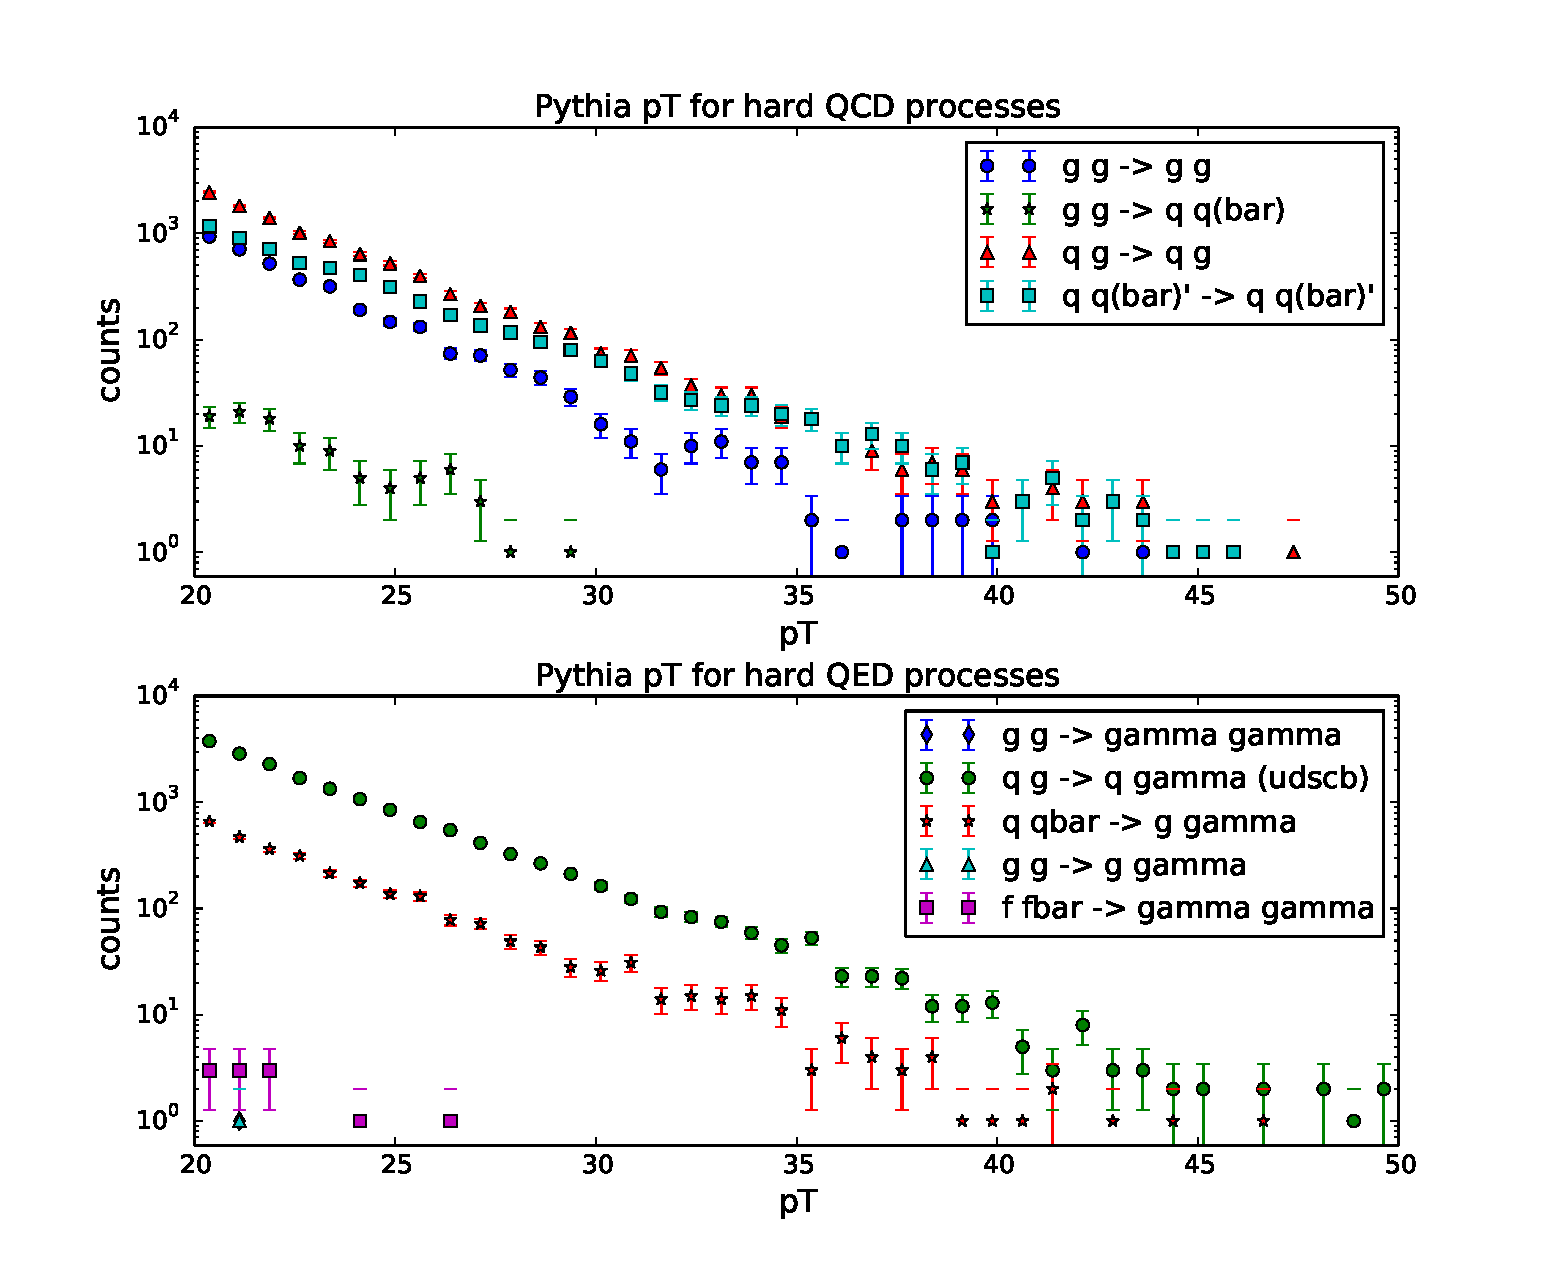
\includegraphics[width=0.9\textwidth]{pT_pythiaEvents.pdf}
\label{fig_label}
\caption{Distribution of jet pT for QCD and QED processes.  Figure created with [python pT\_pythiaEvents.py -m 20000]}
\end{center}
\end{figure}

\begin{figure}[h]
\begin{center}
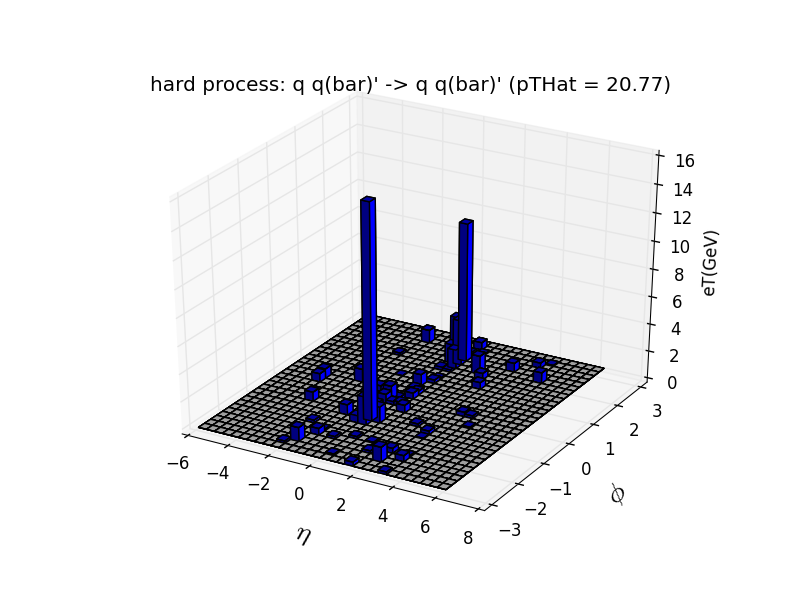
\includegraphics[width=0.49\textwidth]{2d_hist_jetplot.png}
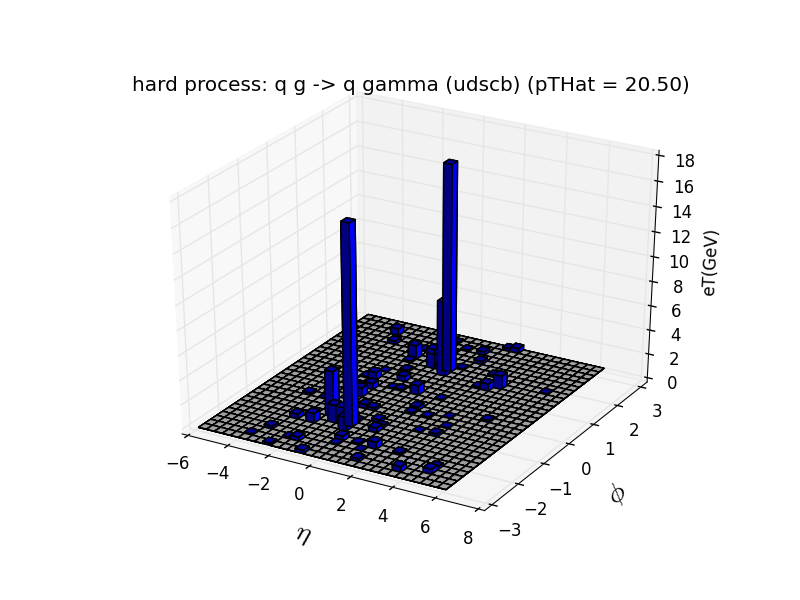
\includegraphics[width=0.49\textwidth]{2d_hist_jetplot2.png}
\label{fig_label}
\caption{Pythia event display for a QCD event, shown to the left, and a QED event shown to the right.  Left figure created with [python 2d\_hist\_jetplot\_wcol.py -o -b 30]. Right figure created with [python 2d\_hist\_jetplot\_wcol.py -o -c -q -b 30]}
\end{center}
\end{figure}

\section{Adding Trento Backgrounds}
%
% Describe how Trento is run, list parameters.
% Describe how we convert Trento output into particle number
% Explain how we generate pT, eta, and phi.
% Explain we add radial flow and elliptic flow from epsilon_2 variable.
%


\begin{figure}[h]
\begin{center}
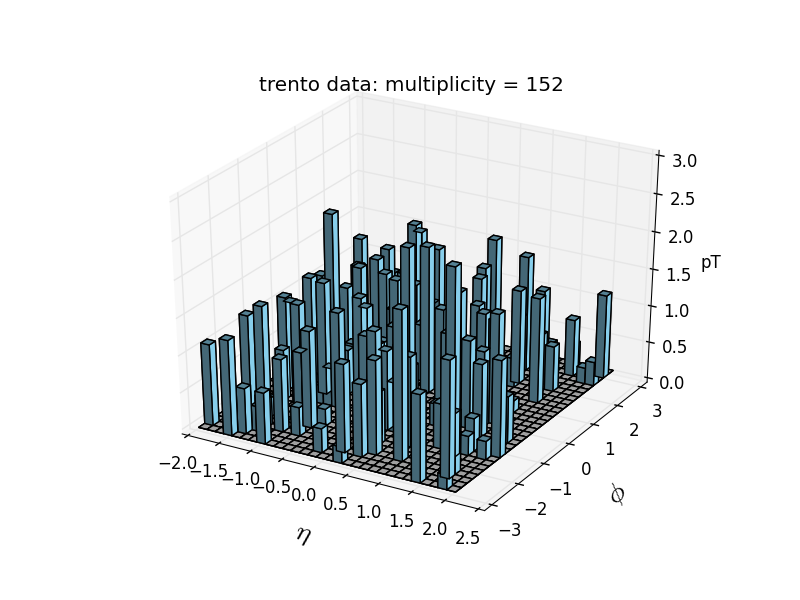
\includegraphics[width=0.9\textwidth]{2d_hist_trento.png}
\label{fig_label}
\caption{Trento event display (no jets).  Figure created with [python 2d\_hist\_trento.py -b 30]}
\end{center}
\end{figure}

\section{Working with SlowJet Finder}
%
% Describe SlowJet Finder algorithm and input parameters.
% Show examples of SlowJet Finder on Pythia only.
% Show example of SlowJet Finder on Pythia plus Trento.
%

\begin{figure}[h]
\begin{center}
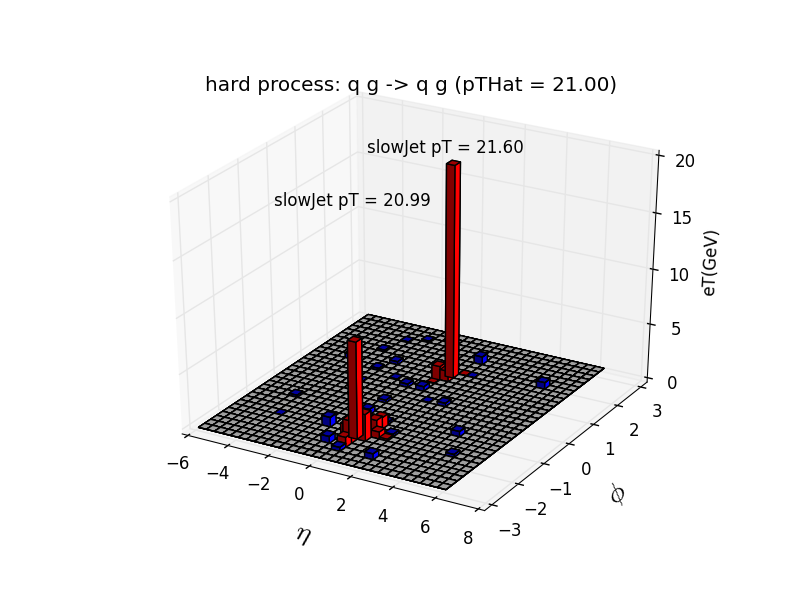
\includegraphics[width=0.9\textwidth]{2d_hist_jetplot_wcol.png}
\label{fig_label}
\caption{Event display for Pythia with SlowJet Finder.  Figure created with [python 2d\_hist\_jetplot\_wcol.py -b 30]}
\end{center}
\end{figure}

\begin{figure}[h]
\begin{center}
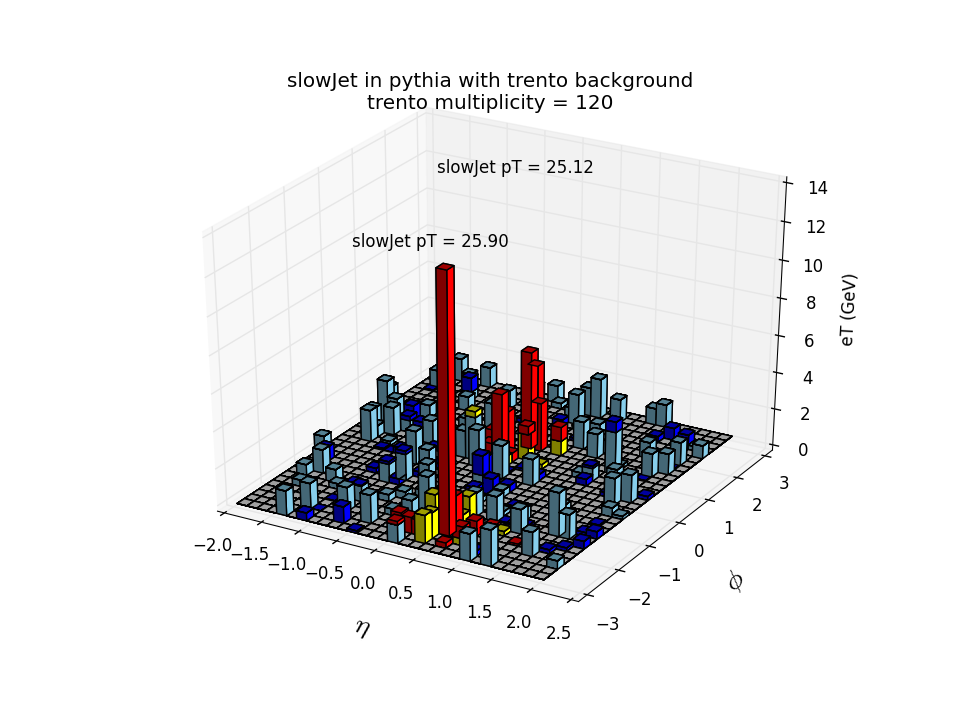
\includegraphics[width=0.9\textwidth]{pythia_slowjet_trento_hist1.png}
\label{fig_label}
\caption{Event display for Pythia+Trento with SlowJet Finder.  Figure created with [python pythia\_slowjet\_trento\_hist.py -b 30 -s 1]}
\end{center}
\end{figure}

\begin{figure}[h]
\begin{center}
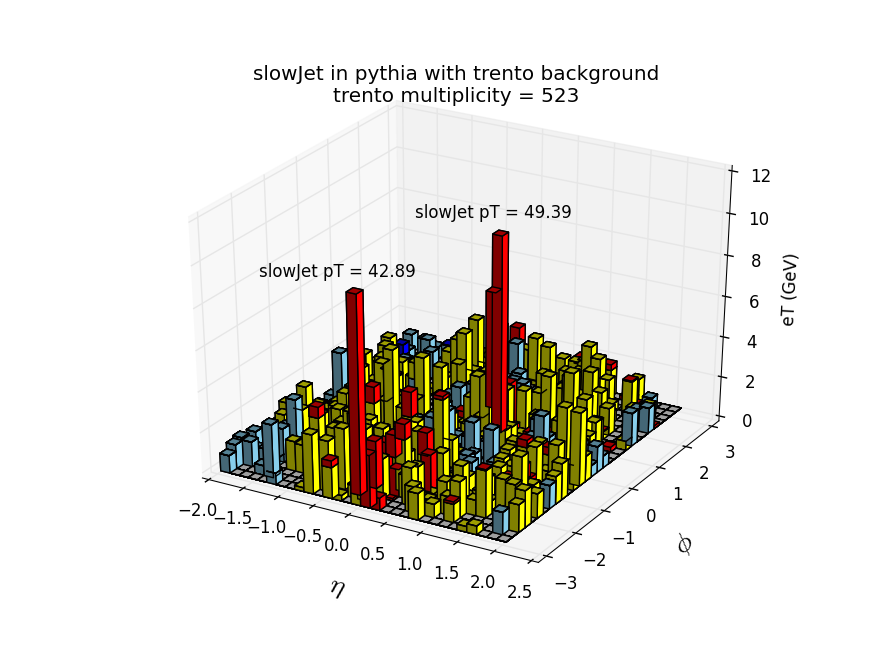
\includegraphics[width=0.9\textwidth]{pythia_slowjet_trento_hist2.png}
\label{fig_label}
\caption{Event display for Pythia+Trento with SlowJet Finder.  Figure created with [python pythia\_slowjet\_trento\_hist.py -b 30 -s 1]}
\end{center}
\end{figure}

\section{Studying Jets}
%
% Define formula for fragmentation function.
% Explain methodology for tracing particles in 
%

\begin{figure}[h]
\begin{center}
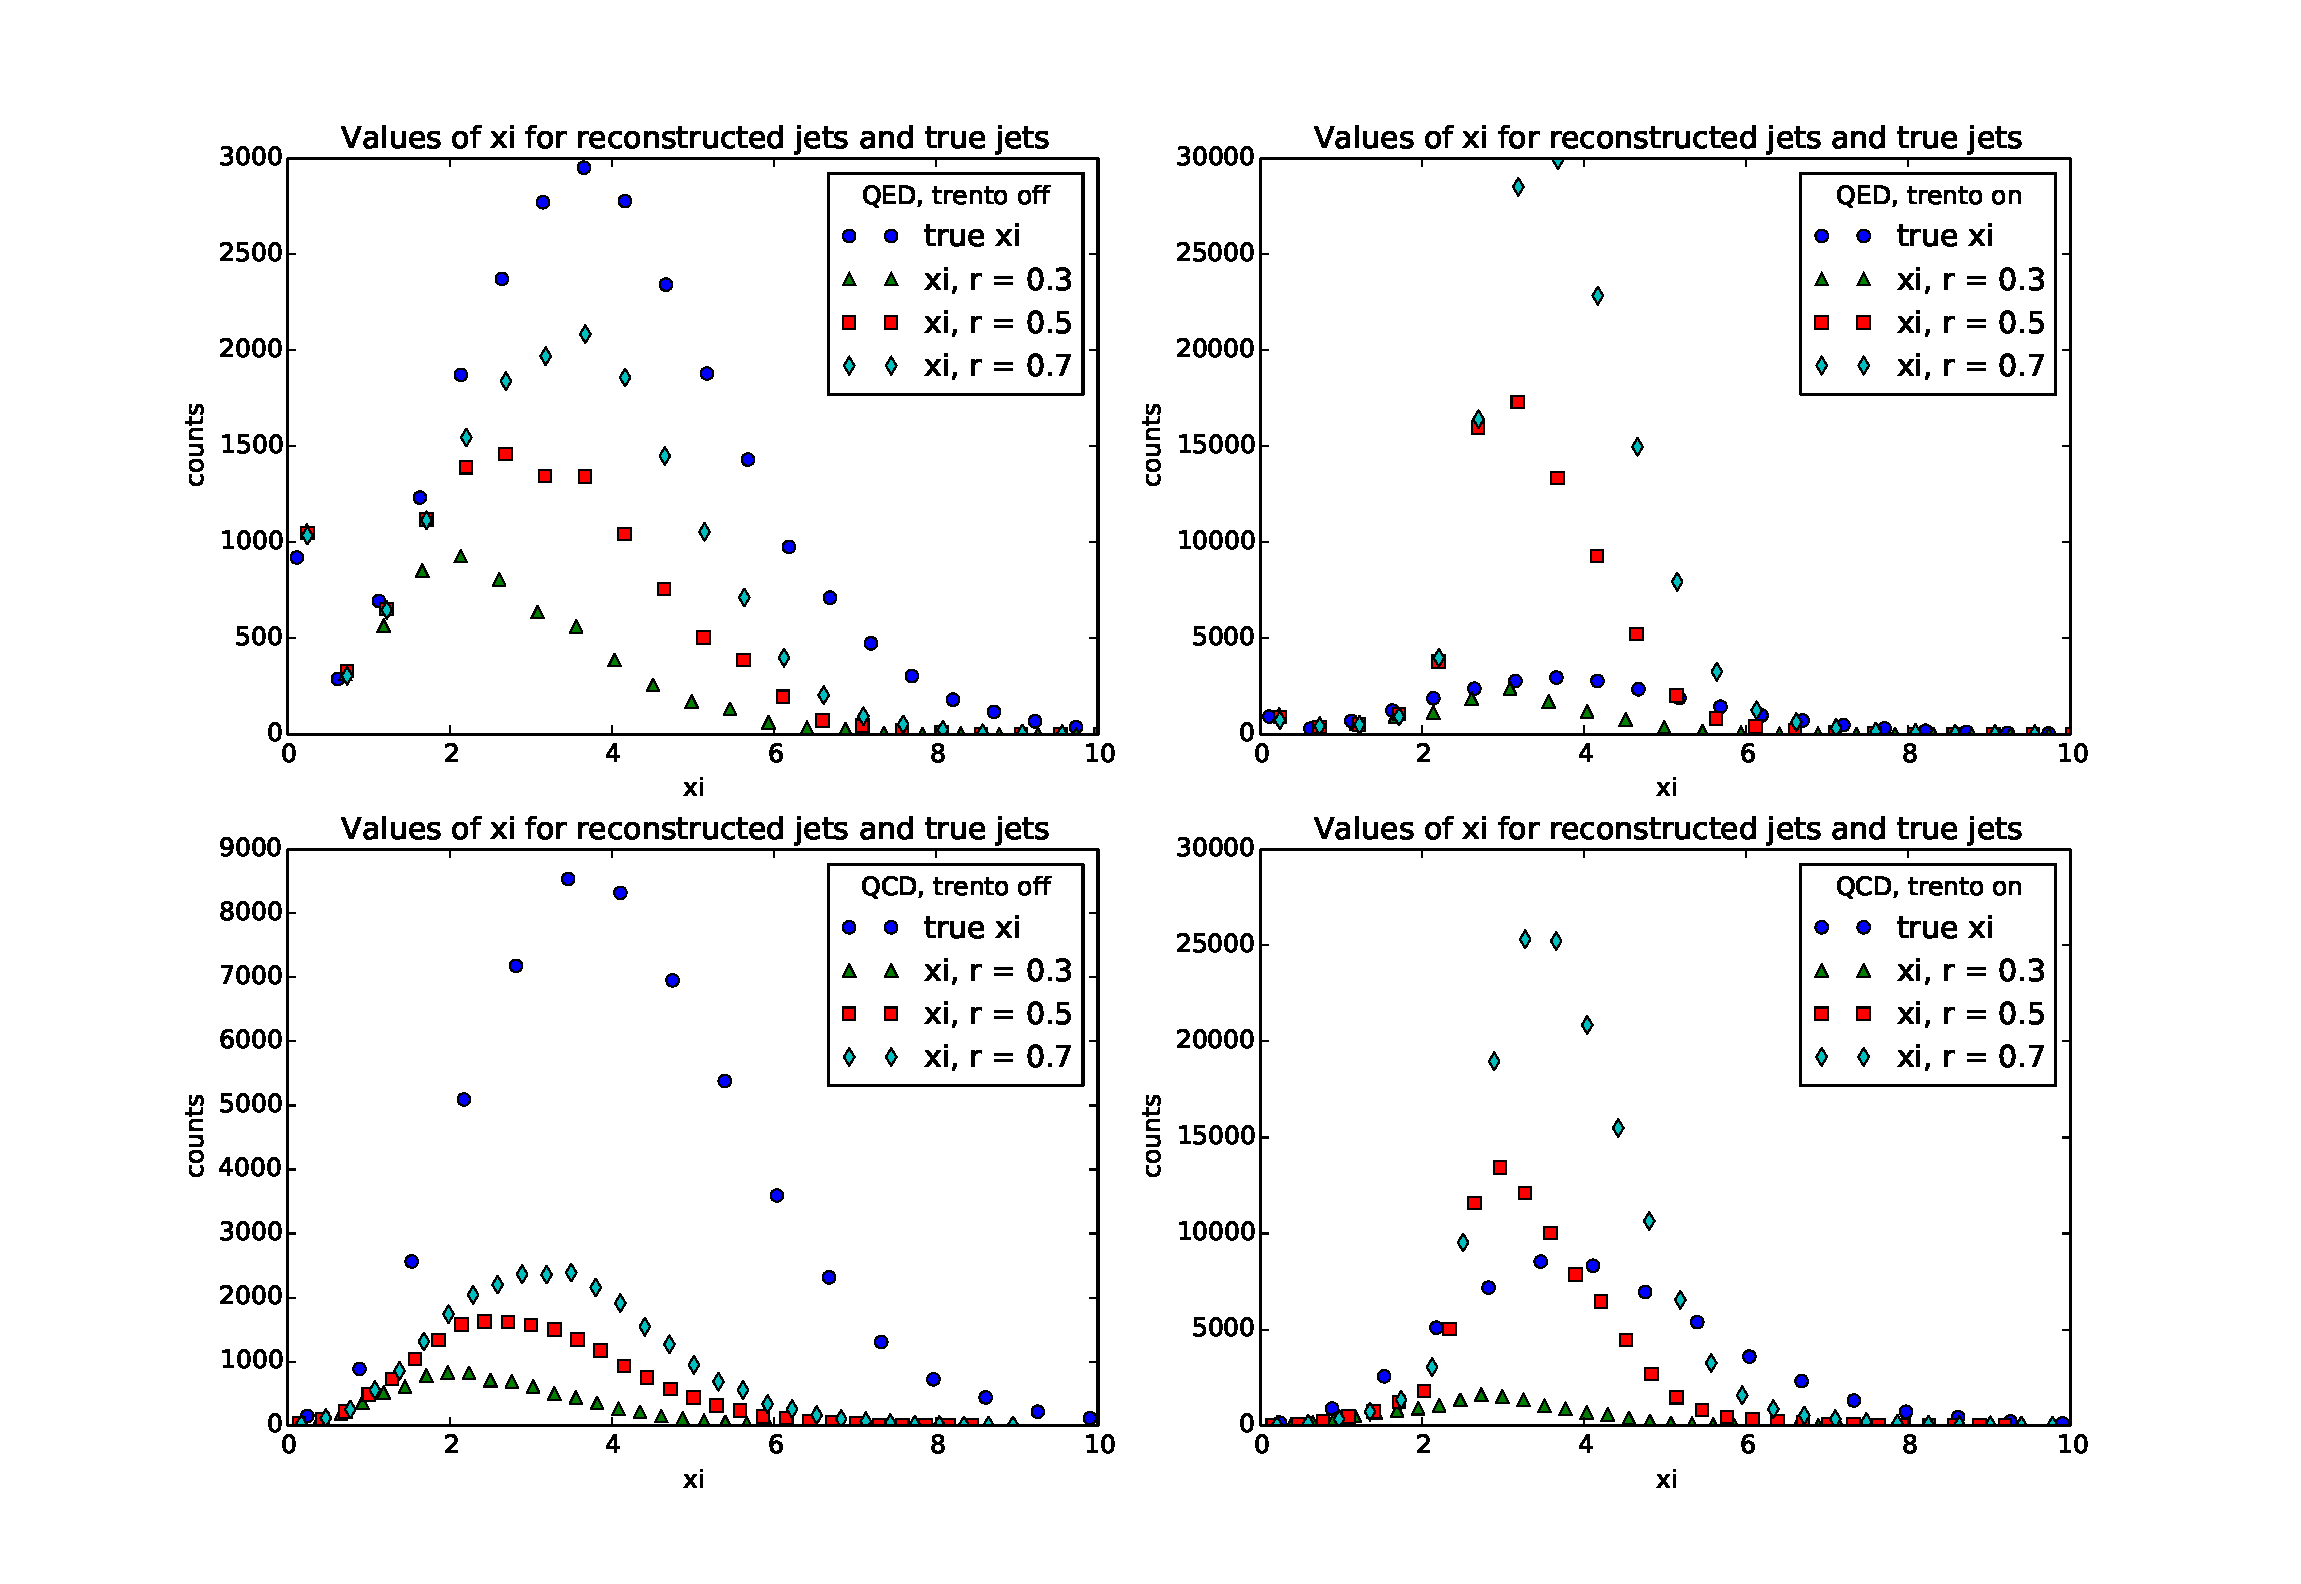
\includegraphics[width=0.9\textwidth]{compare_xi.pdf}
\label{fig_label}
\caption{Fragmentation Function (Xi) distributions for true and reconstructed QCD and QED jets, with and without trento backgrounds.  Figure created with [python compare\_xi.py]}
\end{center}
\end{figure}

\appendix{Listing of Python Scripts}
%
% Provide descriptions for all python scripts, similar to README file.
%

\end{document}